\chapter{Anonymizácia dokumentov}
\label{chap:FirstChapter}

\section{Základné pojmy}
\subsection{Definícia anonymizácie}
\begin{hyphenrules}{nohyphenation}

Anonymizácia je technika ochrany údajov, ktorá zahŕňa odstránenie všetkých identifikačných informácií z osobných údajov tak, aby údaje nebolo možné spojiť s jednotlivcom. Anonymizáciou sa údaje stanú úplne anonymnými a už sa nepovažujú za osobné údaje. Anonymizácia sa často používa v situáciách, keď osobné údaje už nie sú potrebné, ale údaje sa stále môžu použiť na výskumné alebo štatistické účely.\cite{WebPomoc}

\subsection{Typy údajov na anonymizáciu}
Medzi údaje, ktoré sú často predmetom anonymizácie, patria mená, adresy, telefónne čísla, a ďalšie osobné identifikátory. Niektoré údaje majú inú informačnú hodnotu, napríklad, že dátum narodenia osoby je menej cenný než rodné číslo danej osoby. V našom prípade sú anonymizovanými údajmi spravidla kupované predmety a sumy, za ktoré boli predmety kúpené (napr. pri zmluvách ministerstva obrany) a mená a podpisy osôb či firiem, ktoré tieto zmluvy uzavreli.

\subsection{Právne a etické dôvody}

%\todo[inline]{Ak mate jedinu subsection tak asi jej nemusite davat nazov. 
%Vo vacsine pripadov by nemal nasleddovat nadpis subsection hned po nadpise section, skuste tam aspon jednou vetou popisat o co v sekcii ide. Celkovo delit pracu na velmi male celky (subsection o dlzke 2-3 vety) nie je upne vhodne}

Právne predpisy, ako napríklad GDPR v Európskej únii, a etické normy nútia organizácie anonymizovať určité typy údajov. K anonymizácii údajov v Českej republike existuje Zákon o ochrane údajov.\cite{ZakonyProLidi2000-101} Takisto na úrovni Európskej únie existuje smernica upravujúca ochranu fyzických osôb pri spracovaní osobných údajov.\cite{lex-europa} Vzhľadom na skúmané zmluvy a dokumenty je dôležitý zákon č.~412/2005 Sb. o ochraně utajovaných informací a o bezpečnostní způsobilosti.\cite{ZakonyProLidi2005-412}
\section{Metódy a techniky anonymizácie}
\subsection{Manuálne vs. digitálne metódy}
V našej práci rozlišujeme medzi manuálnou a digitálnou anonymizáciou. Manuálna anonymizácia je založená na princípe ručného odstránenia či prelepenia fyzickej zmluvy (obr. 1.1 vľavo), a digitálnymi úpravami, ako je napríklad editácia PDF dokumentu pridaním čierneho obdĺžnika či zašumením pixelov v danej oblasti, ktorá má byť anonymizovaná (obr. 1.1 vpravo.)
\begin{figure}[h]
\begin{minipage}[t]{.45\linewidth}
\fbox{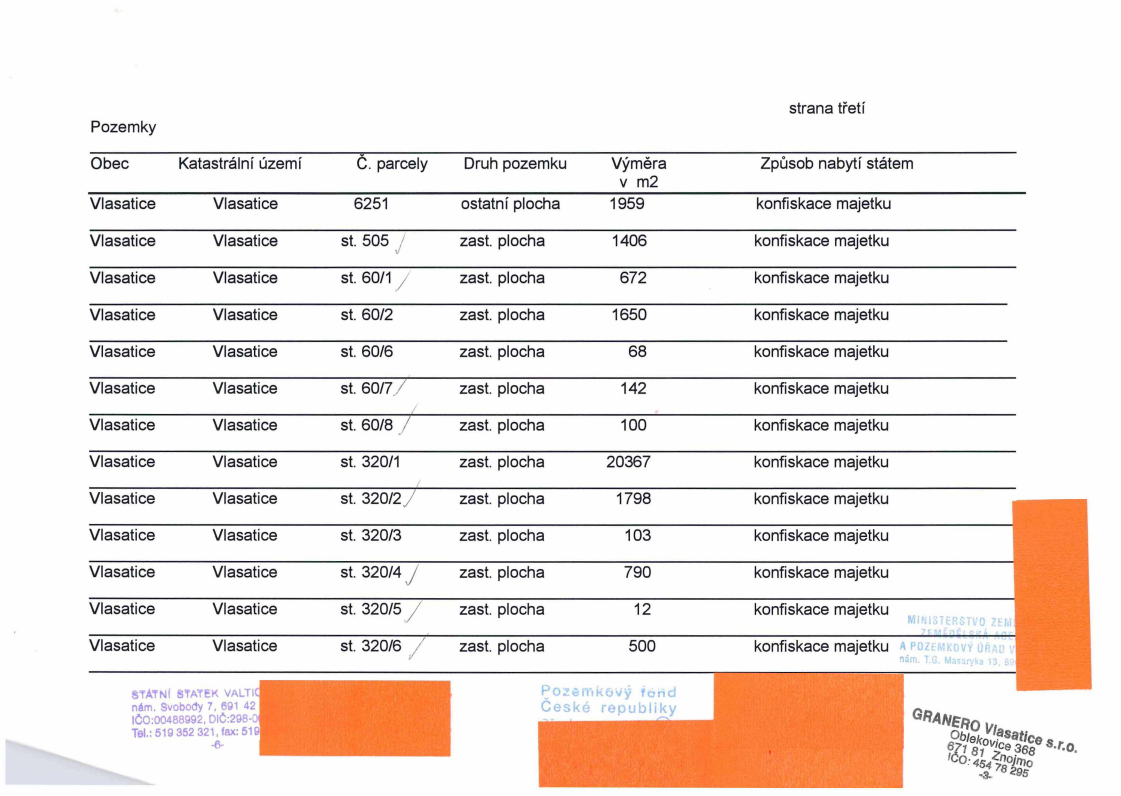
\includegraphics[width=0.9\linewidth]{img/798.png}}
\caption{Porovnanie medzi manuálnou (vľavo) a~digitálnou anonymizáciou (vpravo).}
\end{minipage}\hfill
\begin{minipage}[b]{.45\linewidth}
\fbox{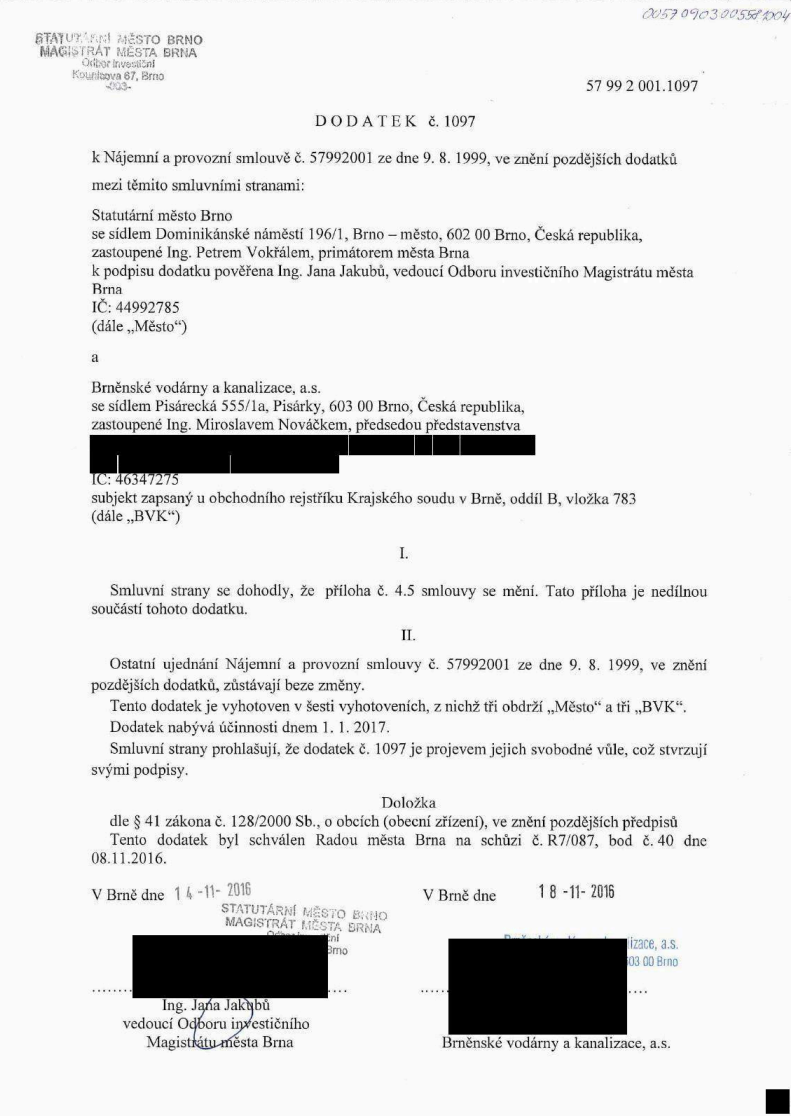
\includegraphics[width=0.9\linewidth]{img/838.png}}
\end{minipage}
\label{fig:1.1}
\end{figure}
\subsection{Technologické nástroje}
Nástroje, ktoré umožňujú automaticky odstraňovať podpisy, časové pečiatky a~iné dôverné informácie, a ich výber závisia od konkrétnych požiadaviek a objemu dokumentov, ktoré je potrebné anonymizovať. Medzi najznámejšie patrí softvér Signer od spoločnosti Software602 \cite{soft602} alebo softvér Syntho \cite{synthoai}. Moderné nástroje ako spomínaný Syntho využívajú technológiu AI na detegovanie údajov, ktoré je potrebné anonymizovať. 
\newline

Medzi kľúčové vlastnosti týchto nástrojov patrí najmä odstránenie osobných údajov, podpisov či časových pečiatok priamo z metadát dokumentov a možnosť označiť a prekryť určité časti dokumentu.

Vo verejnej správe v Českej republike je používaný nástroj, ktorý je priamo pod správou Ministerství vnitra ČR \cite{anonymizace-gov}. Tento nástroj umožňuje vyššie spomínané funkcionality a je jedným z najčastejších spôsobov anonymizácie dokumentov, ktoré v tejto práci riešime.
\end{hyphenrules}
